\section{Fizyka i matematyka lotu}

\begin{frame}{Siły i Wektory - Wiatr jako wyzwanie}
    W idealnym świecie drony latałyby po idealnie prostych liniach. W rzeczywistości przeszkadza im wiatr. Wiatr to z punktu widzenia matematyki nic innego jak \textbf{wektor}.
    
    \vspace{0.5cm}
    \begin{center}
    \begin{tikzpicture}[scale=1.5]
        \draw[thick, ->, blue] (0,0) -- (2,1) node[midway, above left]{Prędkość drona $\vec{V_d}$};
        \draw[thick, ->, red] (2,1) -- (3,0) node[midway, above right]{Wiatr $\vec{W}$};
        \draw[thick, ->, dashed, green!50!black] (0,0) -- (3,0) node[midway, below]{Rzeczywisty tor lotu $\vec{V_{rz}}$};
    \end{tikzpicture}
    \end{center}
    \vspace{0.2cm}
    $\vec{V_{rz}} = \vec{V_d} + \vec{W}$. By utrzymać kurs, dron musi korygować swój lot.
\end{frame}

\begin{frame}{Trajektorie - krzywe parametryczne}
    Do płynnego lotu, np. nagrywania kamerą obiektu w centrum, drony poruszają się po okręgach lub innych kształtach. Do ich opisania używamy równań krzywych.
    
    \vspace{0.3cm}
    \textbf{Przykład - Lot po krzywej w kształcie serca:}
    \begin{columns}
        \begin{column}{0.5\textwidth}
            \small
            Używamy równań parametrycznych (zmienna $t$ od $0$ do $2\pi$):
            \begin{align*}
                x(t) &= 16 \sin^3(t) \\
                y(t) &= 13 \cos(t) - 5 \cos(2t) \\
                     &\quad - 2 \cos(3t) - \cos(4t)
            \end{align*}
            Komputer pokładowy dzieli tę krzywą na mniejsze odcinki i wysyła je jako kolejne współrzędne (waypointy) w formacie geograficznym (LAT/LON).
        \end{column}
        \begin{column}{0.5\textwidth}
            \begin{center}
            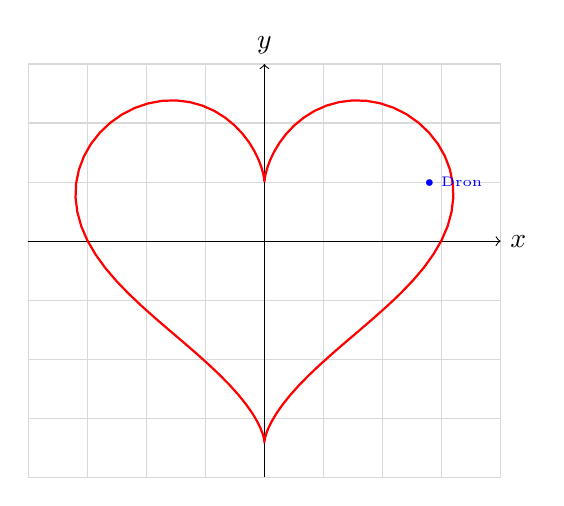
\begin{tikzpicture}[scale=0.15]
                \draw[gray!30, thin, step=5] (-20,-20) grid (20,15);
                \draw[->] (-20,0) -- (20,0) node[right]{$x$};
                \draw[->] (0,-20) -- (0,15) node[above]{$y$};
                
                \draw[thick, red, domain=0:2*pi, samples=100, variable=\t] 
                    plot ({16*sin(\t r)^3}, {13*cos(\t r) - 5*cos(2*\t r) - 2*cos(3*\t r) - cos(4*\t r)});
                
                \node[blue, font=\tiny] at (16, 5) {$\bullet$ Dron};
            \end{tikzpicture}
            \end{center}
        \end{column}
    \end{columns}
\end{frame}

\begin{frame}{Dyskretyzacja trajektorii}
    Aby dron mógł wykonać lot, ciągła funkcja matematyczna musi zostać zamieniona na \textbf{punkty orientacyjne (waypointy)}.
    Dzielimy czas $t$ na równe interwały $\Delta t$.
    
    \vspace{0.3cm}
    \begin{columns}
        \begin{column}{0.5\textwidth}
            \small
            Pomiędzy punktami dron porusza się po liniach prostych (najkrótszą drogą). 
            Im gęściej próbkujemy (mniejsze $\Delta t$), tym ruch jest płynniejszy, ale wymaga przesłania do kontrolera lotu większej liczby danych.
            
            \vspace{0.3cm}
            Tutaj krzywą podzielono na 20 równych odcinków czasowych:
            \begin{align*}
                t_i &= i \cdot \Delta t \\
                \Delta t &= \frac{2\pi}{20}
            \end{align*}
        \end{column}
        \begin{column}{0.5\textwidth}
            \begin{center}
            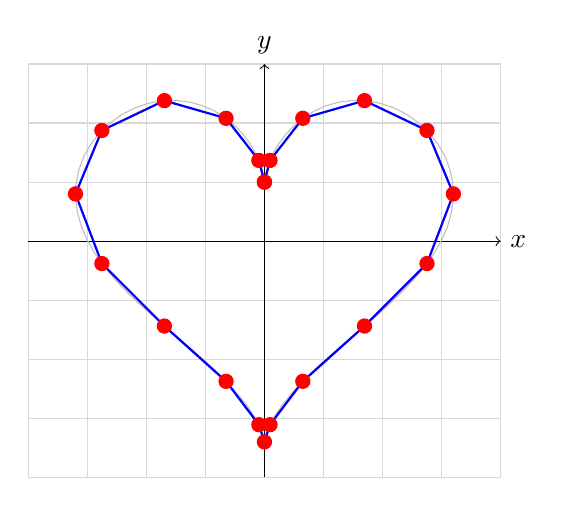
\begin{tikzpicture}[scale=0.15]
                \draw[gray!30, thin, step=5] (-20,-20) grid (20,15);
                \draw[->] (-20,0) -- (20,0) node[right]{$x$};
                \draw[->] (0,-20) -- (0,15) node[above]{$y$};
                
                % Cienka, przezroczysta idealna krzywa w tle
                \draw[gray!50, thin, domain=0:2*pi, samples=100, variable=\t] 
                    plot ({16*sin(\t r)^3}, {13*cos(\t r) - 5*cos(2*\t r) - 2*cos(3*\t r) - cos(4*\t r)});
                    
                % Segmenty linii - zdyskretyzowana trajektoria
                \draw[thick, blue, domain=0:2*pi, samples=21, variable=\t] 
                    plot ({16*sin(\t r)^3}, {13*cos(\t r) - 5*cos(2*\t r) - 2*cos(3*\t r) - cos(4*\t r)});
                
                % Kropki (Waypointy) - wyliczane na podstawie tego samego wzoru
                \foreach \i in {0, 1, ..., 20} {
                    \pgfmathsetmacro{\t}{\i * pi / 10}
                    \pgfmathsetmacro{\x}{16*sin(\t r)^3}
                    \pgfmathsetmacro{\y}{13*cos(\t r) - 5*cos(2*\t r) - 2*cos(3*\t r) - cos(4*\t r)}
                    \filldraw[red] (\x, \y) circle (0.6);
                }
            \end{tikzpicture}
            \end{center}
        \end{column}
    \end{columns}
\end{frame}
